% Options for packages loaded elsewhere
% Options for packages loaded elsewhere
\PassOptionsToPackage{unicode}{hyperref}
\PassOptionsToPackage{hyphens}{url}
%
\documentclass[
  ignorenonframetext,
  aspectratio=169,
  russian,
]{beamer}
\newif\ifbibliography
\usepackage{pgfpages}
\setbeamertemplate{caption}[numbered]
\setbeamertemplate{caption label separator}{: }
\setbeamercolor{caption name}{fg=normal text.fg}
\beamertemplatenavigationsymbolshorizontal
% remove section numbering
\setbeamertemplate{part page}{
  \centering
  \begin{beamercolorbox}[sep=16pt,center]{part title}
    \usebeamerfont{part title}\insertpart\par
  \end{beamercolorbox}
}
\setbeamertemplate{section page}{
  \centering
  \begin{beamercolorbox}[sep=12pt,center]{section title}
    \usebeamerfont{section title}\insertsection\par
  \end{beamercolorbox}
}
\setbeamertemplate{subsection page}{
  \centering
  \begin{beamercolorbox}[sep=8pt,center]{subsection title}
    \usebeamerfont{subsection title}\insertsubsection\par
  \end{beamercolorbox}
}
% Prevent slide breaks in the middle of a paragraph
\widowpenalties 1 10000
\raggedbottom
\AtBeginPart{
  \frame{\partpage}
}
\AtBeginSection{
  \ifbibliography
  \else
    \frame{\sectionpage}
  \fi
}
\AtBeginSubsection{
  \frame{\subsectionpage}
}
\usepackage{iftex}
\ifPDFTeX
  \usepackage[T1]{fontenc}
  \usepackage[utf8]{inputenc}
  \usepackage{textcomp} % provide euro and other symbols
\else % if luatex or xetex
  \usepackage{unicode-math} % this also loads fontspec
  \defaultfontfeatures{Scale=MatchLowercase}
  \defaultfontfeatures[\rmfamily]{Ligatures=TeX,Scale=1}
\fi
\usepackage{lmodern}

\ifPDFTeX\else
  % xetex/luatex font selection
\fi
% Use upquote if available, for straight quotes in verbatim environments
\IfFileExists{upquote.sty}{\usepackage{upquote}}{}
\IfFileExists{microtype.sty}{% use microtype if available
  \usepackage[]{microtype}
  \UseMicrotypeSet[protrusion]{basicmath} % disable protrusion for tt fonts
}{}


\usepackage{longtable,booktabs,array}
\usepackage{calc} % for calculating minipage widths
\usepackage{caption}
% Make caption package work with longtable
\makeatletter
\def\fnum@table{\tablename~\thetable}
\makeatother
\usepackage{graphicx}
\makeatletter
\newsavebox\pandoc@box
\newcommand*\pandocbounded[1]{% scales image to fit in text height/width
  \sbox\pandoc@box{#1}%
  \Gscale@div\@tempa{\textheight}{\dimexpr\ht\pandoc@box+\dp\pandoc@box\relax}%
  \Gscale@div\@tempb{\linewidth}{\wd\pandoc@box}%
  \ifdim\@tempb\p@<\@tempa\p@\let\@tempa\@tempb\fi% select the smaller of both
  \ifdim\@tempa\p@<\p@\scalebox{\@tempa}{\usebox\pandoc@box}%
  \else\usebox{\pandoc@box}%
  \fi%
}
% Set default figure placement to htbp
\def\fps@figure{htbp}
\makeatother



\ifLuaTeX
\usepackage[bidi=basic,provide=*]{babel}
\else
\usepackage[bidi=default,provide=*]{babel}
\fi
% get rid of language-specific shorthands (see #6817):
\let\LanguageShortHands\languageshorthands
\def\languageshorthands#1{}


\setlength{\emergencystretch}{3em} % prevent overfull lines

\providecommand{\tightlist}{%
  \setlength{\itemsep}{0pt}\setlength{\parskip}{0pt}}



 

\usepackage[]{csquotes}

\IfFileExists{plex-otf.sty}{
  %% Full TeXlive
  % \usepackage[%
  %   % math,
  %   RM={Scale=0.94},SS={Scale=0.94},SScon={Scale=0.94},TT={Scale=MatchLowercase,FakeStretch=0.9},DefaultFeatures={Ligatures=Common}
  % ]{plex-otf}
}{
  %% TinyTeX
  \usepackage{libertine}
}

%%% Load theme
% https://deic.uab.cat/~iblanes/beamer_gallery/
\IfFileExists{beamerthemegotham.sty}{
  %% Full TeXlive
  \usetheme{gotham}
  \gothamset{
    numbering=totalpagenumber,
    parttocframe default=off,
    sectiontocframe default=off,
    subsectiontocframe default=off,
  }
}{
  %% TinyTeX
  \usetheme{Madrid}
}
\makeatletter
\@ifpackageloaded{caption}{}{\usepackage{caption}}
\AtBeginDocument{%
\ifdefined\contentsname
  \renewcommand*\contentsname{Содержание}
\else
  \newcommand\contentsname{Содержание}
\fi
\ifdefined\listfigurename
  \renewcommand*\listfigurename{Список иллюстраций}
\else
  \newcommand\listfigurename{Список иллюстраций}
\fi
\ifdefined\listtablename
  \renewcommand*\listtablename{Список таблиц}
\else
  \newcommand\listtablename{Список таблиц}
\fi
\ifdefined\figurename
  \renewcommand*\figurename{Рисунок}
\else
  \newcommand\figurename{Рисунок}
\fi
\ifdefined\tablename
  \renewcommand*\tablename{Таблица}
\else
  \newcommand\tablename{Таблица}
\fi
}
\@ifpackageloaded{float}{}{\usepackage{float}}
\floatstyle{ruled}
\@ifundefined{c@chapter}{\newfloat{codelisting}{h}{lop}}{\newfloat{codelisting}{h}{lop}[chapter]}
\floatname{codelisting}{Список}
\newcommand*\listoflistings{\listof{codelisting}{Листинги}}
\makeatother
\makeatletter
\makeatother
\makeatletter
\@ifpackageloaded{caption}{}{\usepackage{caption}}
\@ifpackageloaded{subcaption}{}{\usepackage{subcaption}}
\makeatother

\usepackage{bookmark}
\IfFileExists{xurl.sty}{\usepackage{xurl}}{} % add URL line breaks if available
\urlstyle{same}
\hypersetup{
  pdflang={ru-RU},
  hidelinks,
  pdfcreator={LaTeX via pandoc}}


\author{}
\date{}

\begin{document}

\renewcommand*\contentsname{Содержание}
\begin{frame}[allowframebreaks]
  \frametitle{Содержание}
  \setcounter{tocdepth}{1}
  \tableofcontents
\end{frame}
\setcounter{tocdepth}{1}
\tableofcontents
}

\begin{frame}
title: \enquote{Лабораторная работа №1} subtitle: \enquote{Операционные
системы} author: \enquote{Исупова Кристина Павловна} institute:
\enquote{Российский университет дружбы народов} date: \enquote{07 марта
2026} format: revealjs
\end{frame}

\begin{frame}
\end{frame}

\section{Информация}\label{ux438ux43dux444ux43eux440ux43cux430ux446ux438ux44f}

\begin{frame}{Докладчик}
\phantomsection\label{ux434ux43eux43aux43bux430ux434ux447ux438ux43a}
\begin{columns}[c]
\begin{column}{0.7\linewidth}
\begin{itemize}[<+->]
\tightlist
\item
  Исупова Кристина Павловна
\item
  Студент НКАбд-05-25
\item
  я Кристина
\item
  Российский университет дружбы народов
\item
  \href{mailto:1132250426@pfur.ru}{\nolinkurl{1132250426@pfur.ru}}
\end{itemize}
\end{column}

\begin{column}{0.3\linewidth}
\pandocbounded{
\includegraphics[keepaspectratio]{./image/kulyabov.jpg}}
\end{column}
\end{columns}
\end{frame}

\begin{frame}
\end{frame}

\section{Цель
работы}\label{ux446ux435ux43bux44c-ux440ux430ux431ux43eux442ux44b}

\begin{frame}{Цель работы}
Приобретение практических навыков взаимодействия пользователя с системой
посредством командной строки.
\end{frame}

\begin{frame}
\end{frame}

\section{Задание}\label{ux437ux430ux434ux430ux43dux438ux435}

\begin{frame}{Задание}
. Определите полное имя вашего домашнего каталога. Далее относительно
этого ката- лога будут выполняться последующие упражнения. 2. Выполните
следующие действия: 2.1. Перейдите в каталог /tmp. 2.2. Выведите на
экран содержимое каталога /tmp. Для этого используйте команду ls с
различными опциями. Поясните разницу в выводимой на экран информации.
2.3. Определите, есть ли в каталоге /var/spool подкаталог с именем cron?
2.4. Перейдите в Ваш домашний каталог и выведите на экран его
содержимое. Опре- делите, кто является владельцем файлов и подкаталогов?
3. Выполните следующие действия: 3.1. В домашнем каталоге создайте новый
каталог с именем newdir. 3.2. В каталоге \textasciitilde/newdir создайте
новый каталог с именем morefun. 3.3. В домашнем каталоге создайте одной
командой три новых каталога с именами letters, memos, misk. Затем
удалите эти каталоги одной командой. 3.4. Попробуйте удалить ранее
созданный каталог \textasciitilde/newdir командой rm. Проверьте, был ли
каталог удалён. 3.5. Удалите каталог \textasciitilde/newdir/morefun из
домашнего каталога. Проверьте, был ли каталог удалён. 4. С помощью
команды man определите, какую опцию команды ls нужно использо- вать для
просмотра содержимое не только указанного каталога, но и подкаталогов,
входящих в него. 5. С помощью команды man определите набор опций команды
ls, позволяющий отсорти- ровать по времени последнего изменения
выводимый список содержимого каталога с развёрнутым описанием файлов. 6.
Используйте команду man для просмотра описания следующих команд: cd,
pwd, mkdir, rmdir, rm. Поясните основные опции этих команд. 7. Используя
информацию, полученную при помощи команды history, выполните мо-
дификацию и исполнение нескольких команд из буфера команд.
\end{frame}

\begin{frame}
\end{frame}

\section{Теоретическое
введение}\label{ux442ux435ux43eux440ux435ux442ux438ux447ux435ux441ux43aux43eux435-ux432ux432ux435ux434ux435ux43dux438ux435}

\begin{frame}{Теоретическое введение}
В операционной системе типа Linux взаимодействие пользователя с системой
обычно осуществляется с помощью командной строки посредством построчного
ввода команд. При этом обычно используется командные интерпретаторы
языка shell: /bin/sh; /bin/csh; /bin/ksh. Формат команды. Командой в
операционной системе называется записанный по специальным правилам текст
(возможно с аргументами), представляющий собой указание на выполнение
какой-либо функций (или действий) в операционной системе.Обычно первым
словом идёт имя команды, остальной текст --- аргументы или опции,
конкретизирующие действие. Общий формат команд можно представить
следующим образом:
\end{frame}

\begin{frame}
\end{frame}

\section{Выполнение лабораторной
работы}\label{ux432ux44bux43fux43eux43bux43dux435ux43dux438ux435-ux43bux430ux431ux43eux440ux430ux442ux43eux440ux43dux43eux439-ux440ux430ux431ux43eux442ux44b}

\begin{frame}{Выполнение лабораторной работы}
Вывожу путь к домашнему каталогу, смотрю содержимое каталога tmp.
(\textbf{?@fig-001})

\begin{figure}

{\centering 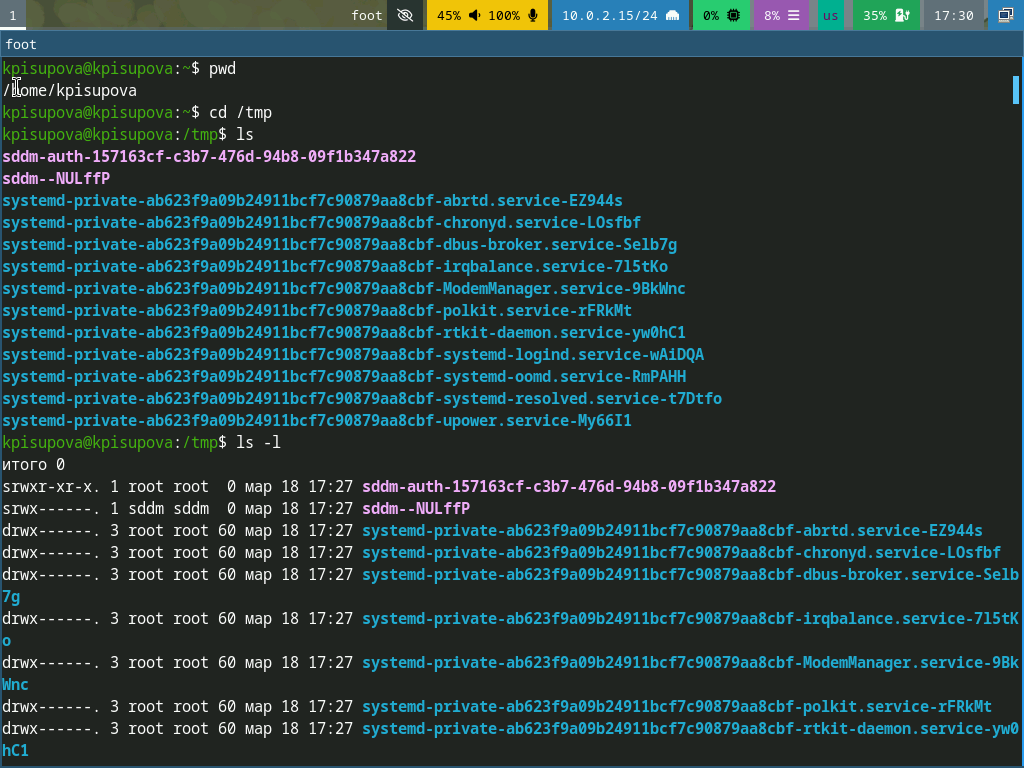
\includegraphics[width=0.7\linewidth,height=\textheight,keepaspectratio]{image/4.1.png}

}

\caption{tmp и домашний каталог}

\end{figure}%
\end{frame}

\begin{frame}
С разными флагами использую команду ls. (\textbf{?@fig-002})

\begin{figure}

{\centering 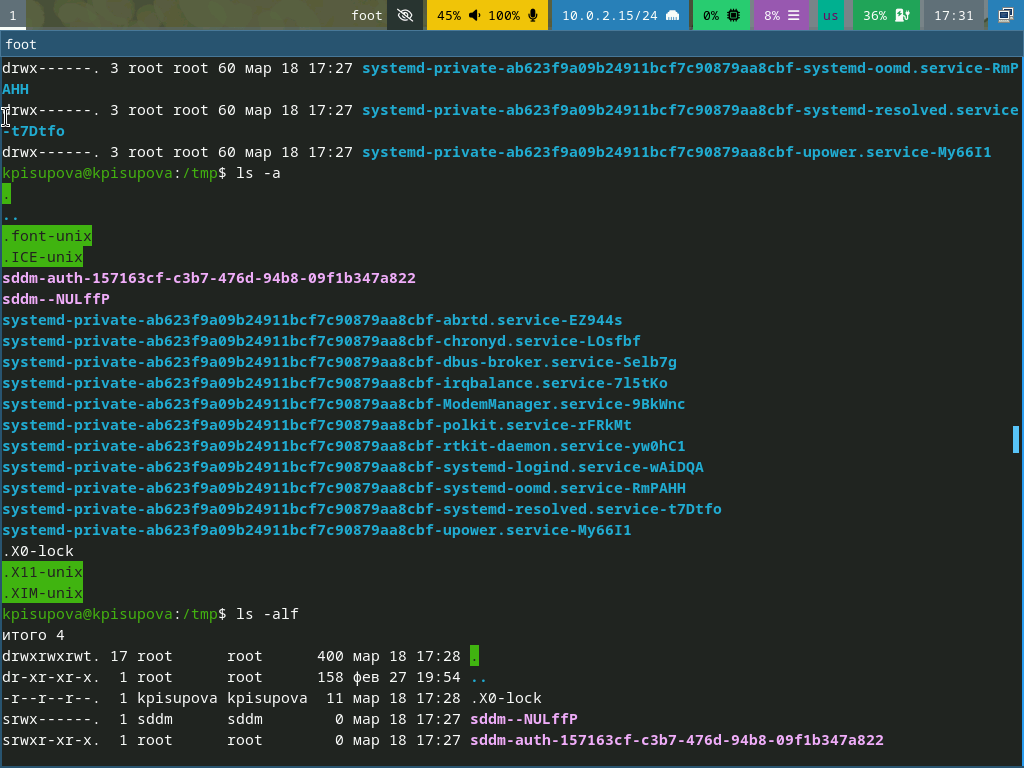
\includegraphics[width=0.7\linewidth,height=\textheight,keepaspectratio]{image/4.2.png}

}

\caption{Использование команды ls}

\end{figure}%
\end{frame}

\begin{frame}
Проверяю, есть ли подкаталог cron в /var/spool. (\textbf{?@fig-003})

\begin{figure}

{\centering 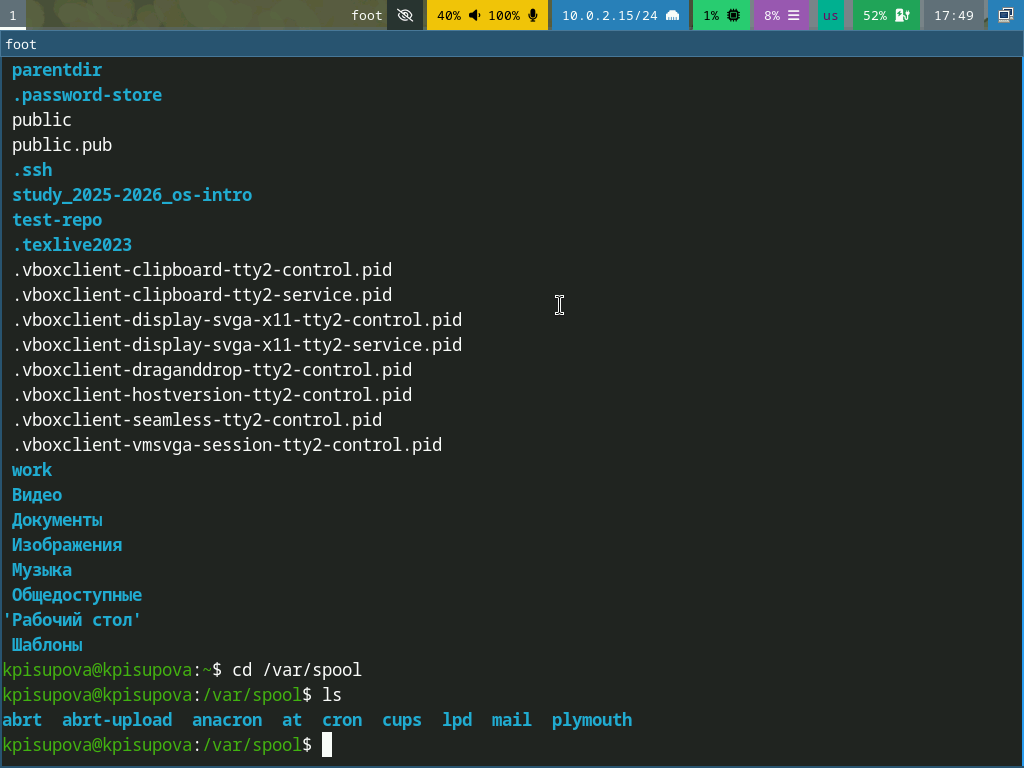
\includegraphics[width=0.7\linewidth,height=\textheight,keepaspectratio]{image/4.3.png}

}

\caption{Проверка подкаталога}

\end{figure}%
\end{frame}

\begin{frame}
Проверяю права доступа в домашнем каталоге. (\textbf{?@fig-004})

\begin{figure}

{\centering 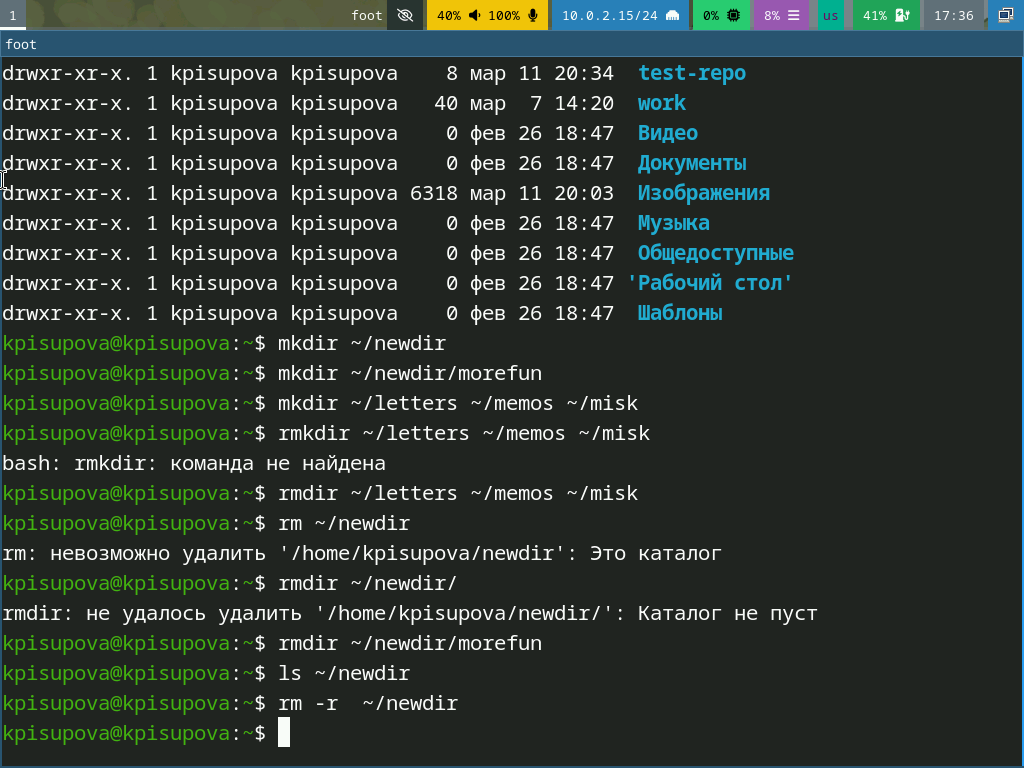
\includegraphics[width=0.7\linewidth,height=\textheight,keepaspectratio]{image/4.4.png}

}

\caption{Права доступа в домашнем каталоге}

\end{figure}%
\end{frame}

\begin{frame}
Играюсь с папками. (\textbf{?@fig-005})

\begin{figure}

{\centering 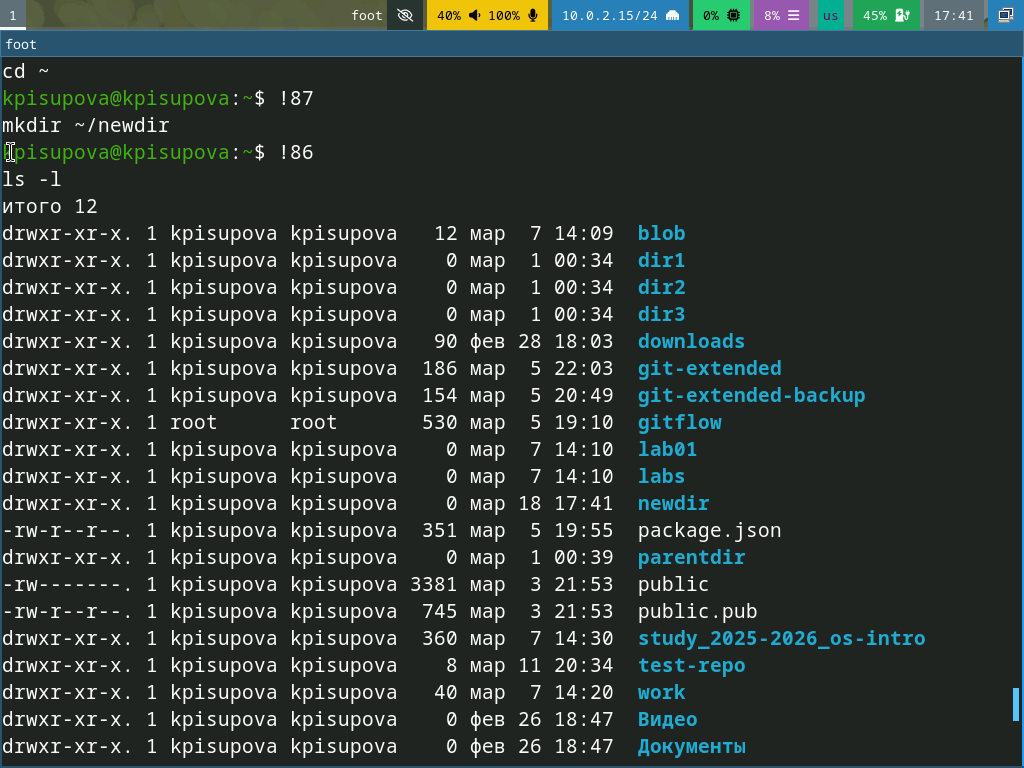
\includegraphics[width=0.7\linewidth,height=\textheight,keepaspectratio]{image/4.5.png}

}

\caption{Создание и удаление каталогов}

\end{figure}%
\end{frame}

\begin{frame}
\end{frame}

\section{Выводы}\label{ux432ux44bux432ux43eux434ux44b}

\begin{frame}{Выводы}
Мы приобрели практические навыки взаимодействия пользователя с системой
посредством командной строки.
\end{frame}

\begin{frame}
\end{frame}




\end{document}
